\chapter{Krav}

På baggrund af et møde med Jim Jensen fra Hammel Neurocenter, som er projektets udbyder, hvor udfordringer med nuværende behandlinger og udredninger af dysfagipatienter blev diskuteret, er der udarbejdet en kravspecifikation til et system kaldet Synkerefleksmonitor (SRM). Formålet med mødet var ikke at etablere kunde/leverandør- relation, hvor krav til et kommende produkt skal forhandles på plads. Mødet havde i stedet en uformel karakter, hvor Hammel Neurocenter frivilligt er gået med til at mødes med gruppens medlemmer for at bidrage med deres ekspertise indenfor behandling og udredning af dysfagipatienter. Kravene til produktet som skal realiseres under dette projekt, er suverænt udspecificeret af gruppens medlemmer uden indblanding af projektets udbyder. Fra udbydernes side var der kun et ønske om at bidrage med udvikling af nye metoder til udredning af dysfagipatienter, hvilken dette projekt også har intentioner om. \\

I det følgende beskrives kort det overordnede system, efterfulgt af funktionelle og ikke funktionelle krav.  

\section{Systembeskrivelse}
Systemet består af et BI kredsløb og en kommerciel EMG-måler, der tilsammen udgør SRM'en, se figur \ref{fig:sysbeskrivelse}. SRM'en initieres af et sundhedspersonale ved første at tilkoble elektroder fra hhv. BI- og EMG-måleren til et raske måleobjekt. Derefter igangsætter sundhedspersonalet målingerne via. en brugergrænseflade på en PC. Begge målinger kører simultant. Efterfølgende opsamles målingerne i en A/D-konverter, der omsætter de målte værdier fra analoge til digitale værdier, som PC'en kan arbejde med. I PC'en processeres de to målinger og vises til sundhedspersonalet via. brugergrænsefladen.   

\begin{figure}[H]
\centering
{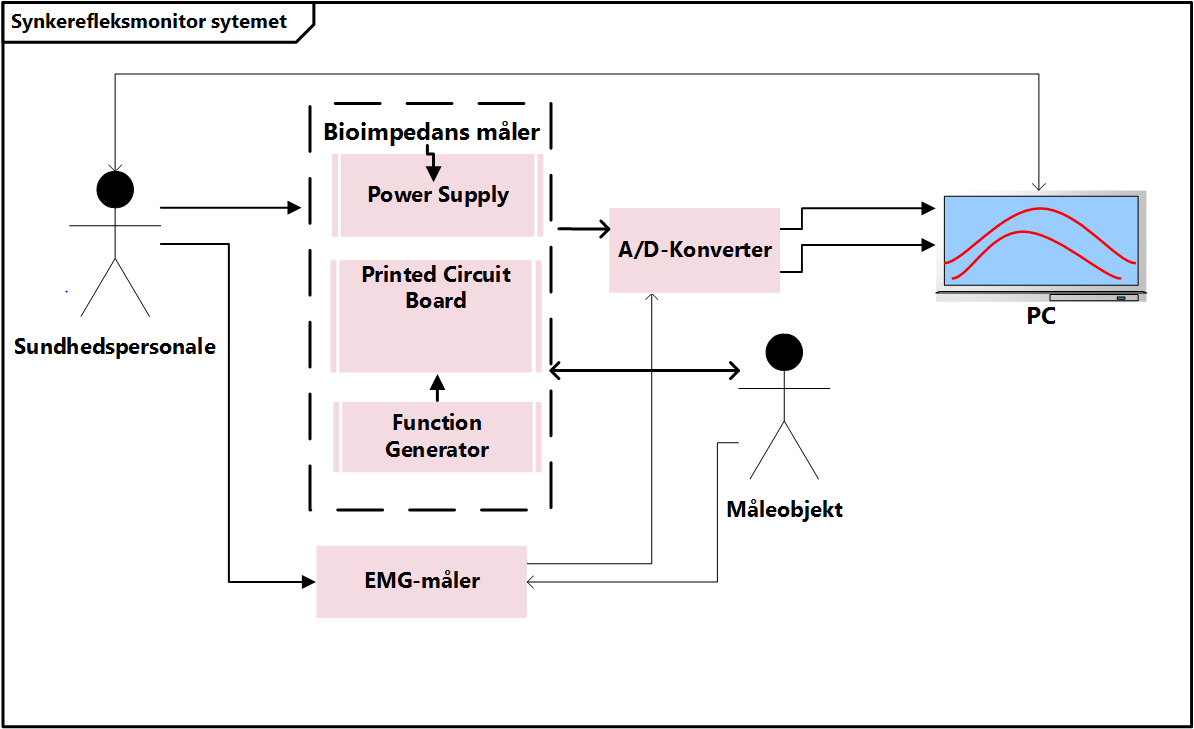
\includegraphics[width=10cm]
{Figure/AktoerKontextDiagram}}
\caption{Aktør-kontekst diagram illustrer det overordnet systemet, som betsår af to måleapparater, en A/D-konverter og en PC. Et sundhedspersonale igangsætter målingerne via. en brugergrænseflade. Måleobjektet er tilkoblet til begge apparater. }
\label{fig:sysbeskrivelse}
\end{figure}  

 

\section{Aktørbeskrivelse}
Til aktør-kontekst diagrammet følger der en en aktør beskrivelse, der beskriver kort hver komponentes funktion, se tabel \ref{tab:aktoerbeskrivelse}.    

\begin{table}[H]
\begin{tabularx}{\textwidth}{l l X}
     Aktørnavn	&	Type		&	Beskrivelse \\ \midrule
     Sundhedspersonale   	&  	Primær  	& 	Sundhedspersonalet tilkobler BI- og EMG-måleren til måleobjektet vha. elektroder, samt starter målingen. Yderligere interagerer sundhedspersonalet med en brugergrænseflade.     \\ 			  \addlinespace[2mm]
     Bioimpedans-måler	&	Sekundær	& BI- måleren anvendes til at måle bioimpedans signaler fra måleobjektet  	 \\   \addlinespace[2mm]

  EMG-måler	&	Sekundær	&	EMG-måleren anvendes til at måle EMG signaler fra måleobjektet.
     \\   \addlinespace[2mm]
    
    Måleobjekt	&	Sekundær	&	Måleobjektet er kilden  hvorfra biosignalerne indhentes. Måleobjektet er tilkoblet til både BI- og EMG-måleren.
     \\   \addlinespace[2mm]
     
 A/D-konverter	&	Sekundær	&	A/D-konverterens funktion er at konvertere analoge signaler fra hhv. BI-og EMG-måleren  til digitale signaler.
     \\   \addlinespace[2mm]      
    PC	&	Sekundær	&	Denne brugergrænseflade bruges til at visualisere de målte signaler i graf form.
     \\   \addlinespace[2mm]
     
   
     \bottomrule                                                                                                                   
    \end{tabularx}
    \caption {Aktørbeskrivelse for det samlede system}
    \label{tab:aktoerbeskrivelse}
	
\end{table}


\section{Funktionelle krav}

Tabel \ref{tab:moscow} beskriver funktionelle krav, der stilles til applikationen synkerefleksmonitor. Nogle krav er vigtigere end andre, og de prioriteres vha. MosCow-metoden. Kravene i \textit{Must og Should} kategorien prioriteres højest.  I dette projekt bestræbes det at opfylde kravene i \textit{Must og Should}. Yderligere detaljer om kravspecifikationen henvises til \nameref{bilag1}. Her kan man bl.a. læse ændringer i kravspecifikationen under projektet. 

\begin{table}[H]

\begin{tabularx}{\textwidth}{X|X}
\rowcolor{Gray}
\toprule
\textbf{Must have} & \textbf{Should have} \\
\hline \\
\textbf{1. }Systemet skal have en bioimpedans sensor (BI), der kan måle bioimpedans signaler & \textbf{5. }Matlab GUI, der kan præsentere BI og EMG signaler \\[4ex]
\textbf{2. }Systemet skal have EMG sensor, der kan måle EMG signaler & \textbf{6. }Både BI og EMG målinger skal køre simultant\\[4ex]
\textbf{3. }Systemet skal kunne vise BI og EMG signaler over tid på en graf (offline) i Matlab  & \\[4ex]
\textbf{4. }Systemet skal kunne beregne BI på baggrund af målte spændinger & \\[4ex]


\midrule
    \rowcolor{Gray}
    \textbf{Could have} & \textbf{Would have}\\
    \midrule \\
    \textbf{7. }Validere bioimpedans sensoren op imod kommerciel BI måler & \textbf{10. }Mobilt synkerefleksmonitor med touch skærm\\[4ex]
\textbf{8. }Real-time visning af EMG- og BI signalerne & \textbf{11. }EMG og BI signalerne overføres til EPJ  \\[4ex]
\textbf{9. }Machine Learning for at diskriminere mellem synkerefleks og støj (tale og hoste)& \textbf{12. }Tage højde for anatomiske forskelle mellem kønnene\\[4ex]
& \\

\end{tabularx}

\caption{MoSCoW opdeling af funktionelle krav til  synkerefleksmonitorens software og hardware}
  \label{tab:moscow}
\end{table}

\pagebreak
For at realisere \textit{Must og Should } kravene, er der udviklet use cases, der bidrager til opfyldelsen af disse krav. Brugergrænsefladen til applikationen er forsøgt forsimplet, således at brugeren kun forholder sig til behandlede data og ikke rådata. På Figur \ref{UseCaseV1} ses det to aktører, der interagerer med to use cases.  Herunder beskrives funktionerne af de to use cases. 


\begin{figure}[H]
\centering
{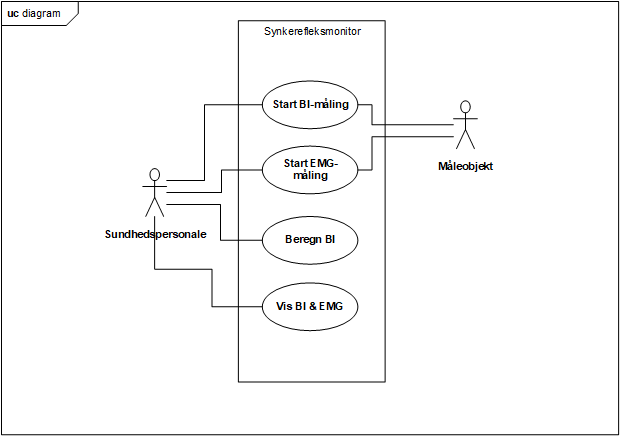
\includegraphics[width=10cm]
{Figure/usecasediagram}}
\caption{UseCase diagram for synkerefleksmonitoren. Systemet består af to usecases, der tilsammen bruges til at starte, måle og gemme BI og EMG målinger}
\label{UseCaseV1}
\end{figure}

\textbf{Use Case - Start Measurements:}
Denne use case bruges til at igangsætte en måling. Når sundhedspersonalet trykker på denne knap, køres der en række funktioner, der til sammen behandler og visualisere to målinger. Funktionaliteten af denne knap implementeres i Matlab. I  \nameref{bilag6} kan du bl.a. læse om de underliggende funktioner, som eksekveres, når denne knap aktiveres af brugeren.\\

\textbf{Use Case - Save Measurements:}
Denne use case muliggør at brugerne kan gemme to målinger lokalt i en csv fil. Her gemmes de to målinger, som brugeren har taget simultant i use casen \textit{"Start Measurements".} \\
 
 
 \pagebreak
Nedenunder er der en fully dressed for \textit{"Start Measurements"} use casen. Her kan du læse de trin som brugeren skal igennem for at igangsætte en måling. Fully dressed for use casen \textit{"Save Measurements"} henvises der til \nameref{bilag1}. 

\textbf{Use Cases - fully dressed  } 


\begin{longtabu} to \linewidth{@{}l r X[l]@{}} %UC1%
	{\large \textbf{Use Case - Start Measurements }} && \\
	\toprule
	Scenarie 				&&	Hovedscenarie\\
	Navn 					&& 	Start Measurements\\
	Mål 					&& 	At måle to signaler simultant \\
	Initiering 				&& 	Startes af Sundhedspersonalet\\
	Aktører 				&& 	Sundhedspersonale (primær)\\
	
	Samtidige forekomster  	&& 	1 måling pr. kørsel \\
	Forudsætninger 			&&	BI-måleren og EMG-måleren er ledige og operationelle. Elektroderne påsat måleobjektet og GUI-vinduet er åbent \\ 
	Resultat 				&& 	To målinger foretages og vises til brugeren\\ \midrule
	Hovedscenarie 			&    1. 	&	Sundhedspersonalet trykker på knappen "Start Measurements "\\				 	
							&    2. 	& 	En række funktioner køres automatisk og systemet sørger for at to målinger foretages simultant\\
	
	
	&&[\textit{Undtagelse 2.a:}] Systemet foretager ikke målinger\\ \midrule						
							
							
	Undtagelser 			&		2.a	& 	Applikationen genstartes og hovedscenarie 1 i use casen gentages \\ \bottomrule
	
	\caption{Fully dressed for use casen \textit{Start Measurements}}
	\label{UC1}
\end{longtabu}

\section{Ikke-funktionelle krav}


